\section{AI-Specific Optimizations}
\label{sec:aiopt}

\subsection{Why General-Purpose NoCs Are Not Enough}

Traditional NoCs were largely designed around general-purpose traffic, but AI workloads have communication patterns that are both more regular and more demanding. Neural networks exhibit heavy one-to-many reuse, irregular sparsity in weights and activations, and heterogeneous precision ranging from FP16 to low-bit integer formats. If a NoC ignores these characteristics, it wastes bandwidth on redundant unicast transfers, sends zero values unnecessarily, and uses fixed-width flits even when data precision has been reduced \cite{chen2019eyerissv2,zhang2016cambriconx}.

The group presentation summarizes this mismatch clearly: general-purpose NoCs assume relatively uniform traffic, while AI workloads create repeated broadcasts, dynamic sparsity, and precision-dependent bandwidth demand. As a result, the NoC is not merely transporting tensors; it is directly participating in the efficiency of dataflow execution.

\subsection{Multicast-Aware Routing}

One key optimization direction is multicast-aware routing. In weight-stationary and input-stationary mappings, one value may need to reach many processing elements. Path-based multicast encodes multiple destinations in the packet header and forks traffic only at branching routers, making it flexible for irregular destinations at the cost of growing header overhead. In the presentation, this approach is described as a natural fit for XY-style routing with destination information carried explicitly in the packet. Tree-based multicast, by contrast, builds a spanning tree ahead of time and carries only a compact tree identifier in each packet. This lowers per-packet overhead and fits static dataflows well, but it is less adaptive when sparsity or routing demand changes at runtime. Both approaches reduce redundant traffic compared with repeated unicasts and are therefore well matched to the broadcast-heavy nature of AI accelerators.

\begin{figure*}[!t]
\centering
\subfloat[Path-based multicast: destinations are encoded in the packet header and forking occurs only at branching routers.\label{fig:pathmulticast}]{%
\begin{minipage}[c][0.25\textheight][c]{0.46\textwidth}
\centering
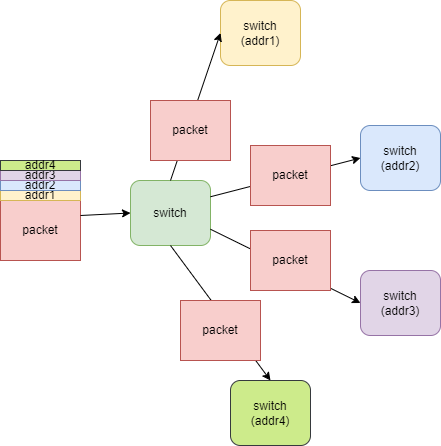
\includegraphics[height=0.23\textheight]{image/fig_path_multicast.png}
\end{minipage}}
\hfill
\subfloat[Tree-based multicast: a preconfigured spanning tree carries only a compact tree identifier in each packet.\label{fig:treemulticast}]{%
\begin{minipage}[c][0.25\textheight][c]{0.46\textwidth}
\centering
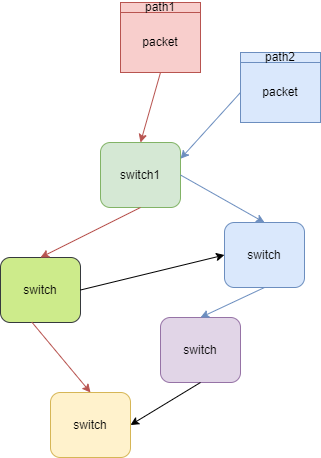
\includegraphics[height=0.23\textheight]{image/fig_tree_multicast.png}
\end{minipage}}
\caption{Comparison of two multicast strategies for AI accelerator NoCs. Path-based multicast (left) provides flexibility for irregular destination sets at the cost of header overhead, while tree-based multicast (right) minimizes per-packet metadata but requires static tree setup.}
\label{fig:multicast}
\end{figure*}

Recent trends further show that multicast support is no longer a binary choice between pure unicast and one fixed tree. Hybrid schemes can mix unicast and multicast phases, while reconfigurable fabrics and sparsity-aware pruning try to preserve the efficiency of multicast without paying the full cost under dynamic workloads. This reinforces the broader theme that AI communication increasingly rewards structure-aware networking rather than generic best-effort packet delivery.

\subsection{In-Network Compression and Sparsity Awareness}

A second major direction is in-network data compression. Sparsity-aware schemes transmit only non-zero values and their coordinates, while precision-aware schemes adapt payload width to the layer's quantization level. Model-aware techniques extend the same intuition to transformer and embedding-heavy systems by reducing communication for low-value or highly reusable data before traffic enters the network. Across these approaches, the common goal is to reduce link bandwidth demand and buffer energy without changing the algorithmic function of the model \cite{zhang2016cambriconx,jouppi2023tpuv4}. The presentation frames this as a direct response to redundancy in AI models: zeros, low-bit values, and repeated data structures all imply that raw tensor traffic is often much larger than the information that truly matters.

In practice, the challenge is that the NoC becomes more workload-aware and therefore more specialized: the better it exploits structure, the harder it may be to retain flexibility across CNNs, transformers, and future model families. AI-specific optimization therefore improves efficiency at the cost of additional router logic, metadata handling, and workload dependence.

\begin{table}[!t]
\caption{AI-Oriented NoC Optimization Directions}
\label{tab:aiopt}
\centering
\footnotesize
\setlength{\tabcolsep}{3pt}
\renewcommand{\arraystretch}{1.08}
\begin{tabularx}{\columnwidth}{p{1.5cm}Y p{1.65cm}}
\toprule
Technique & Role in AI NoCs & Main Trade-Off \\
\midrule
Path multicast & Replicates packets only at branch routers and adapts to irregular one-to-many traffic. & Header grows with fan-out. \\
Tree multicast & Uses preconfigured trees with small packet metadata for stable dataflows. & Static setup; less flexible. \\
Sparse compression & Sends only non-zero values and coordinates to cut link and buffer pressure. & Metadata and decode overhead. \\
Precision compression & Matches traffic volume to low-bit precision or data importance. & Layer-dependent scheduling. \\
\bottomrule
\end{tabularx}
\end{table}

The broader lesson is that AI-specific NoC optimization is not about making routers universally smarter; it is about co-designing communication with workload structure. Once communication is recognized as part of the dataflow, NoC features such as router replication, compression, and traffic scheduling become architectural tools rather than low-level implementation details.
